\documentclass[11pt]{article}
\usepackage[margin=1in]{geometry}
\usepackage{booktabs}
\usepackage{graphicx}
\usepackage{float}
\begin{document}
\section*{Supplementary Step 8 Visualization Report}
\subsection*{Overview}
\begin{tabular}{p{0.42\linewidth}p{0.50\linewidth}}
\toprule
Metric & Value\\
\midrule
Tested concrete-abstract pairs & 225\\
Pairs surviving FDR & 0\\
Matched-pair subset size & 12\\
Matched subset FDR-significant pairs & 0\\
Ranked questions & 30\\
Selected channel-followup pairs & 3\\
\bottomrule
\end{tabular}
\paragraph{Interpretation note.} The exploratory item-pair analysis did not identify any concrete-abstract question pairs with reliable back-ROI differences after Benjamini-Hochberg correction. This supports the view that the back ROI does not show robust item-specific discrimination in the current dataset. The lowest-q pair was 2018\_CH\_77 versus 2021\_CH\_86 (mean difference=1.864e-07, raw p=0.003431, q=0.596248). No matched-pair subset comparison survived FDR correction under the predeclared matching rule.
\paragraph{Top pair summary.} Top descriptive pair: 2018\_CH\_77 versus 2021\_CH\_86 (mean difference=1.864e-07, raw p=0.003431, q=0.596248).
\subsection*{Core Step 8 Heatmaps}
\begin{figure}[H]
\centering
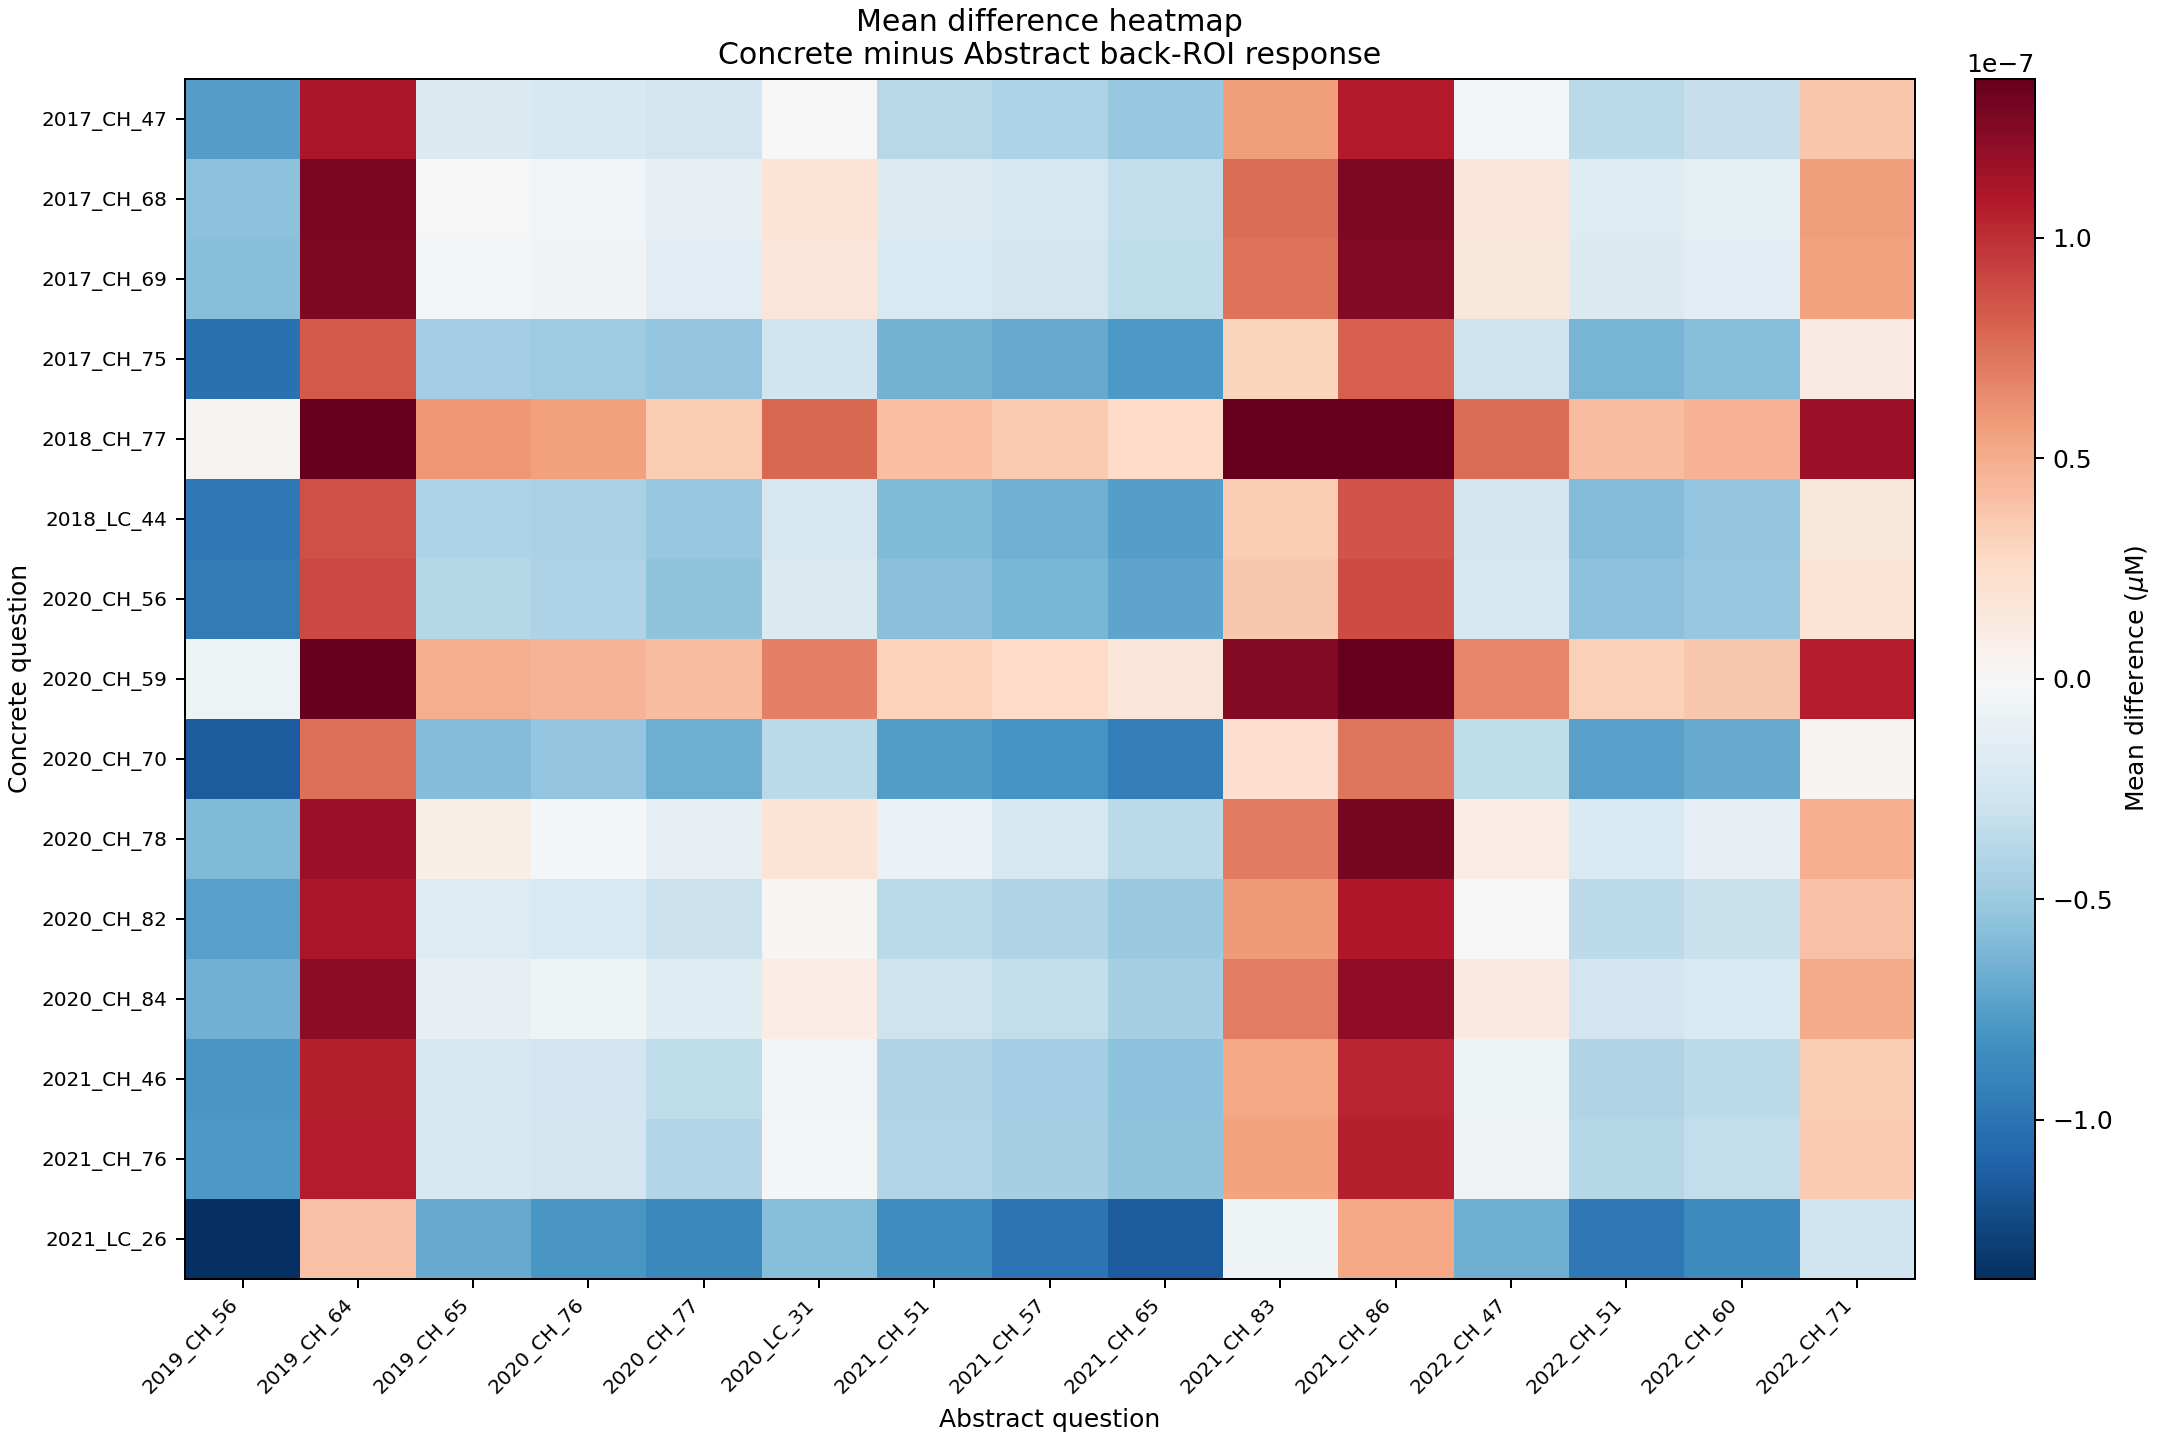
\includegraphics[width=0.95\linewidth]{../../figures/step8/pairwise_mean_difference_heatmap.png}
\caption{Mean back-ROI concrete-minus-abstract differences for all item pairs.}
\end{figure}
\begin{figure}[H]
\centering
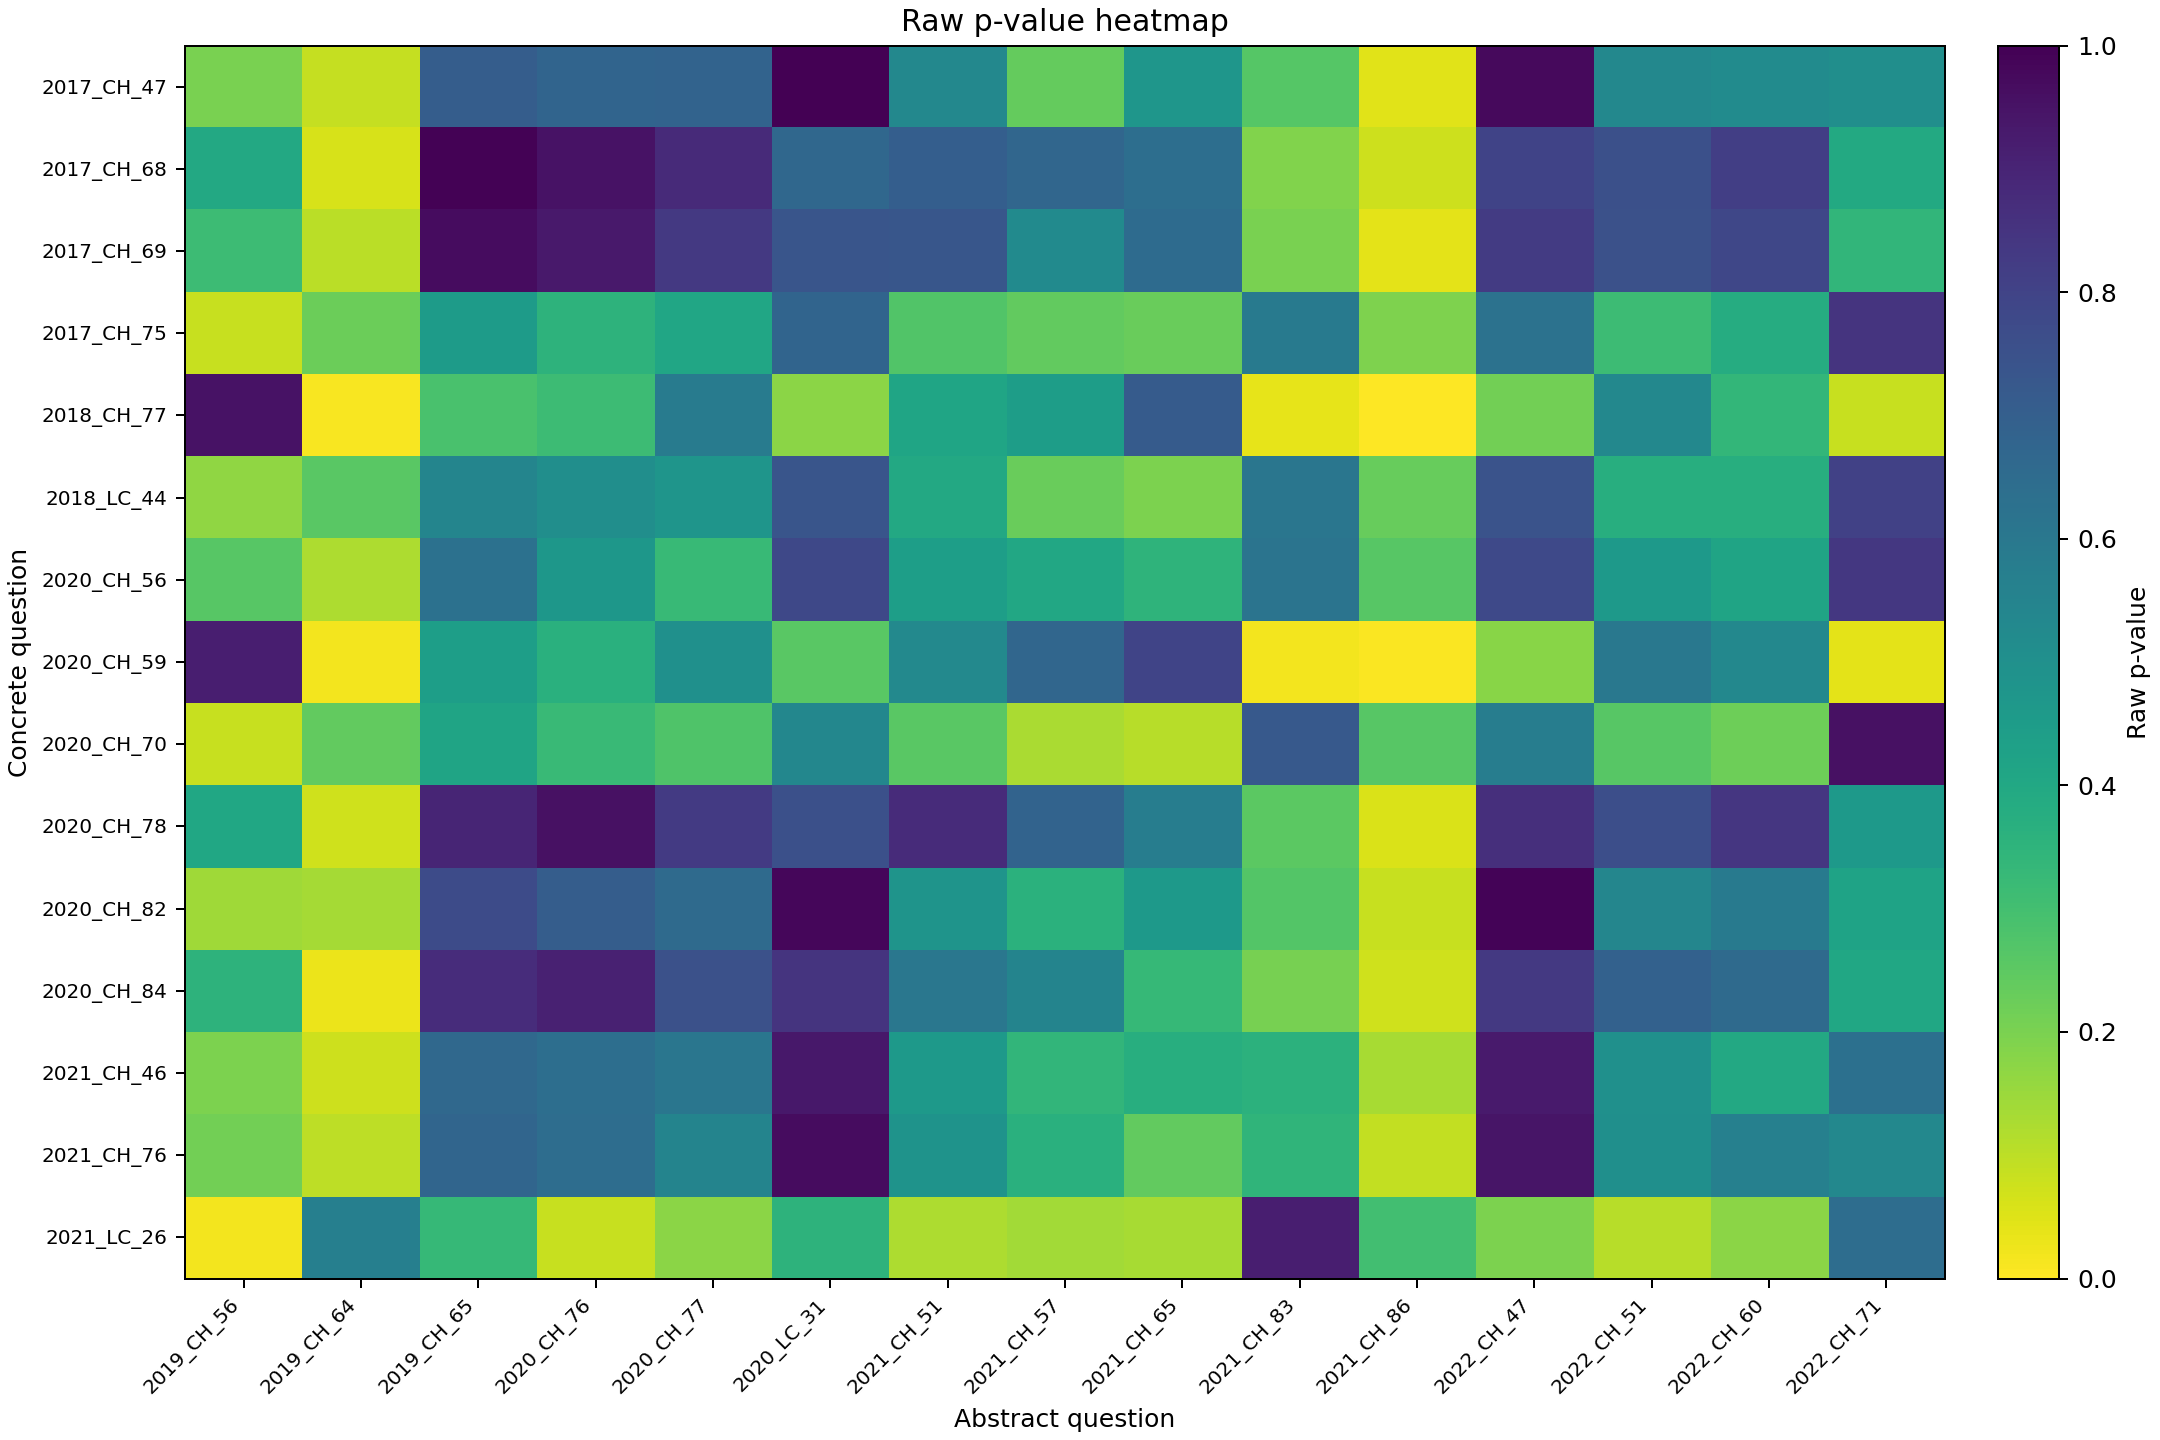
\includegraphics[width=0.48\linewidth]{../../figures/step8/pairwise_raw_pvalue_heatmap.png}
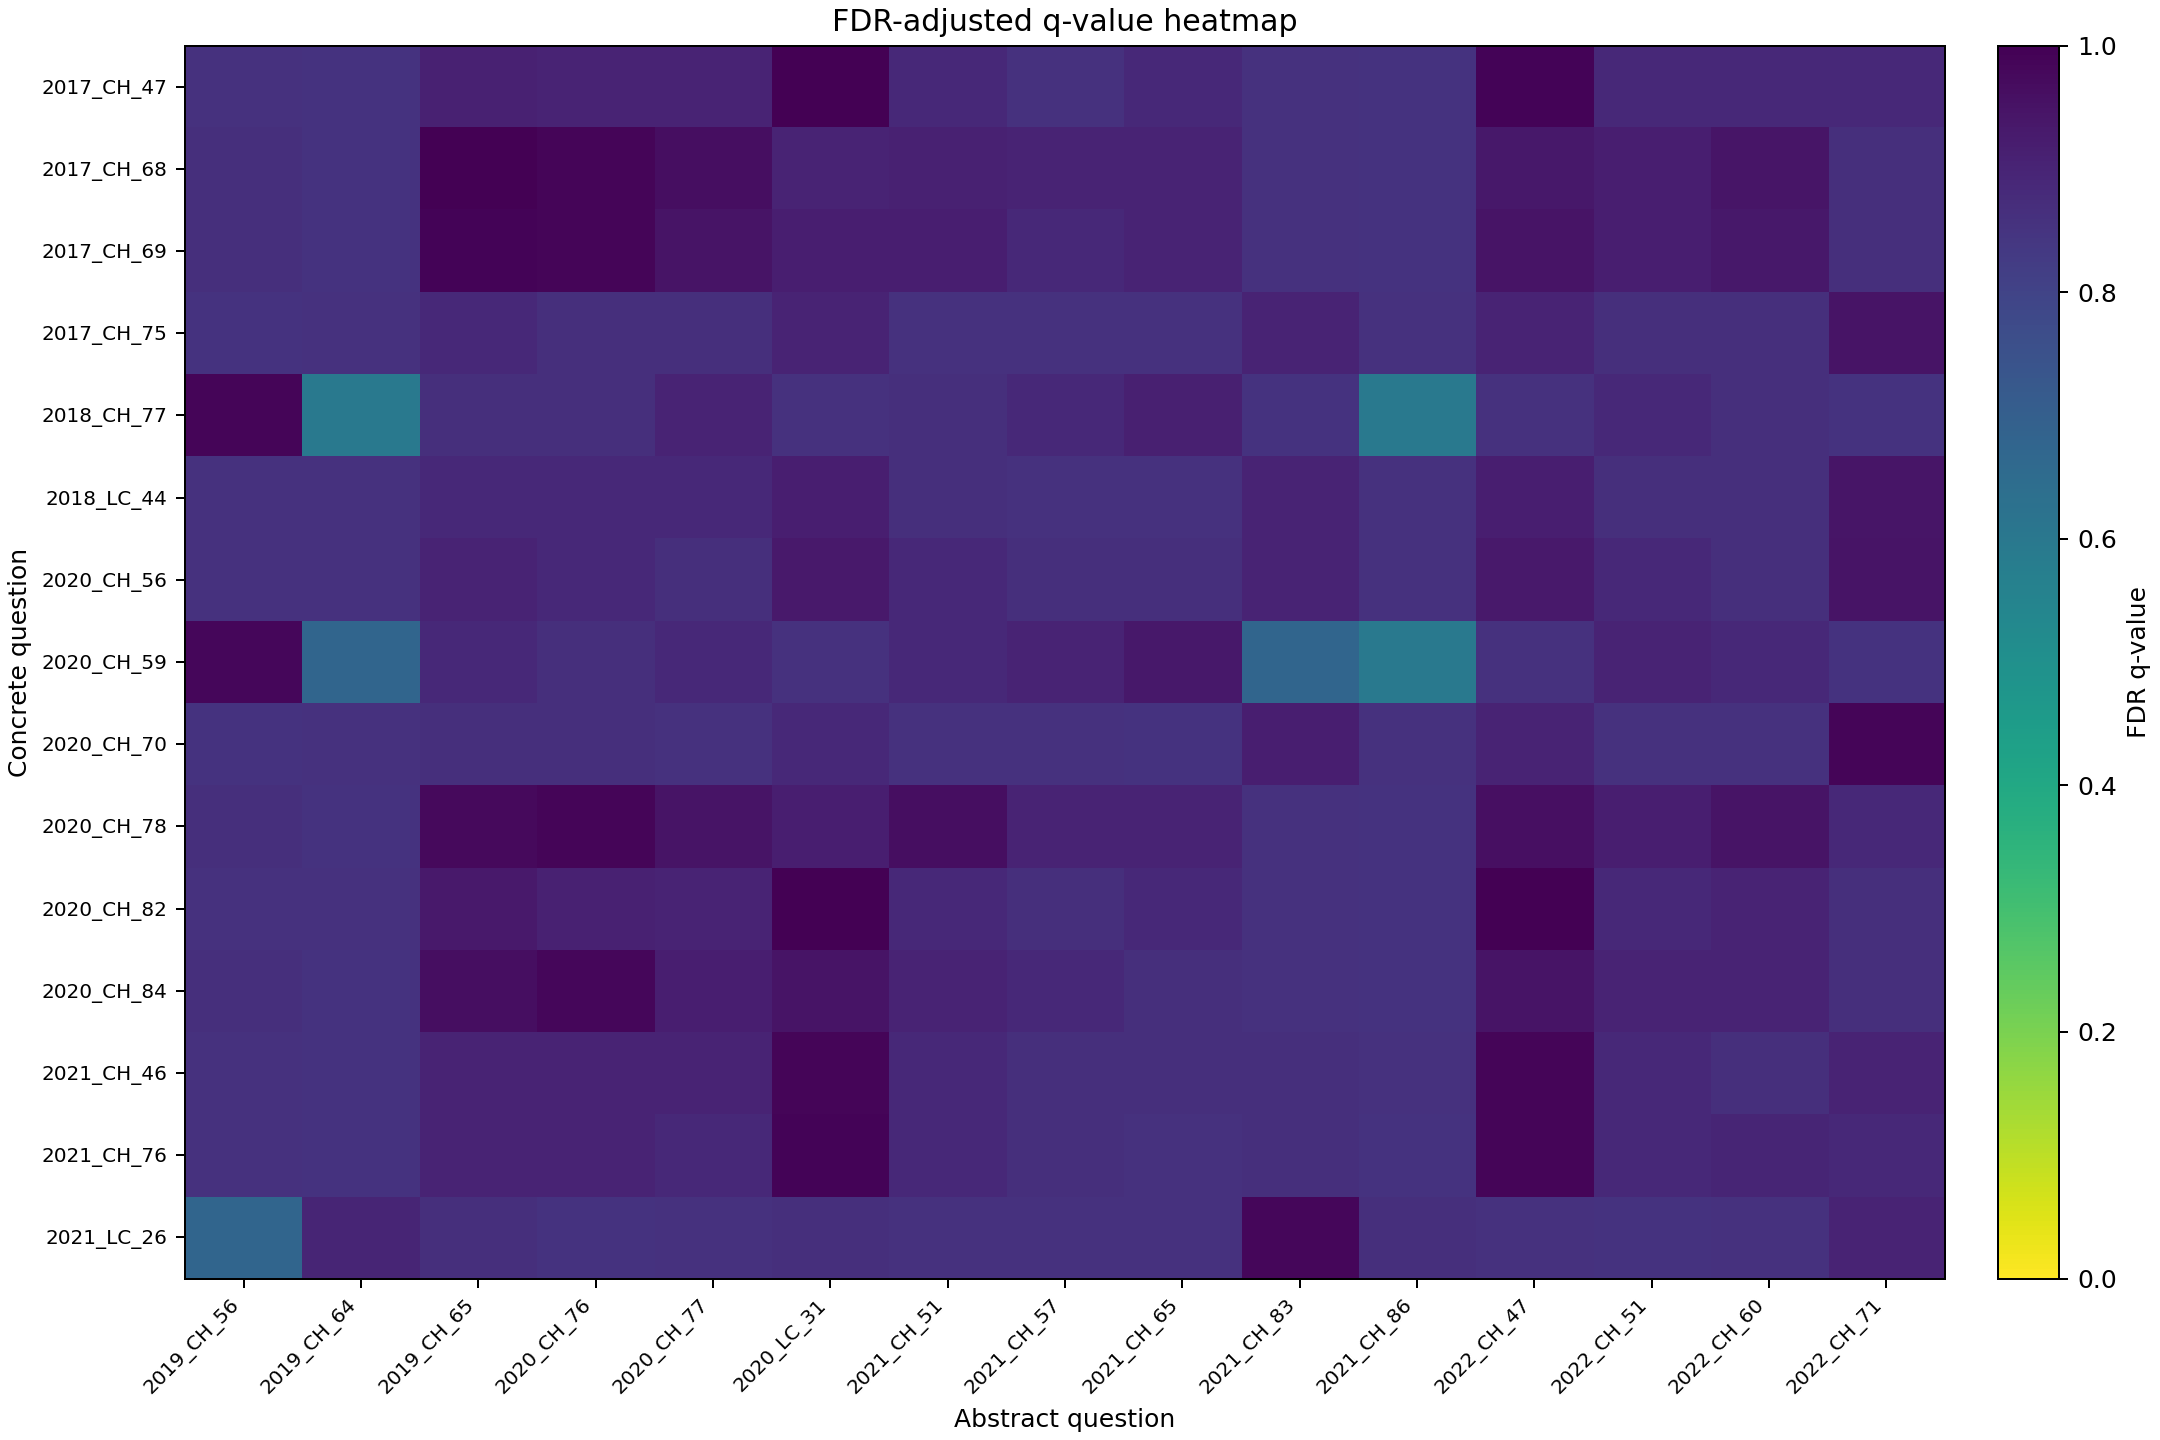
\includegraphics[width=0.48\linewidth]{../../figures/step8/pairwise_fdr_qvalue_heatmap.png}
\caption{Raw p-values and FDR-adjusted q-values across all tested item pairs.}
\end{figure}
\begin{figure}[H]
\centering
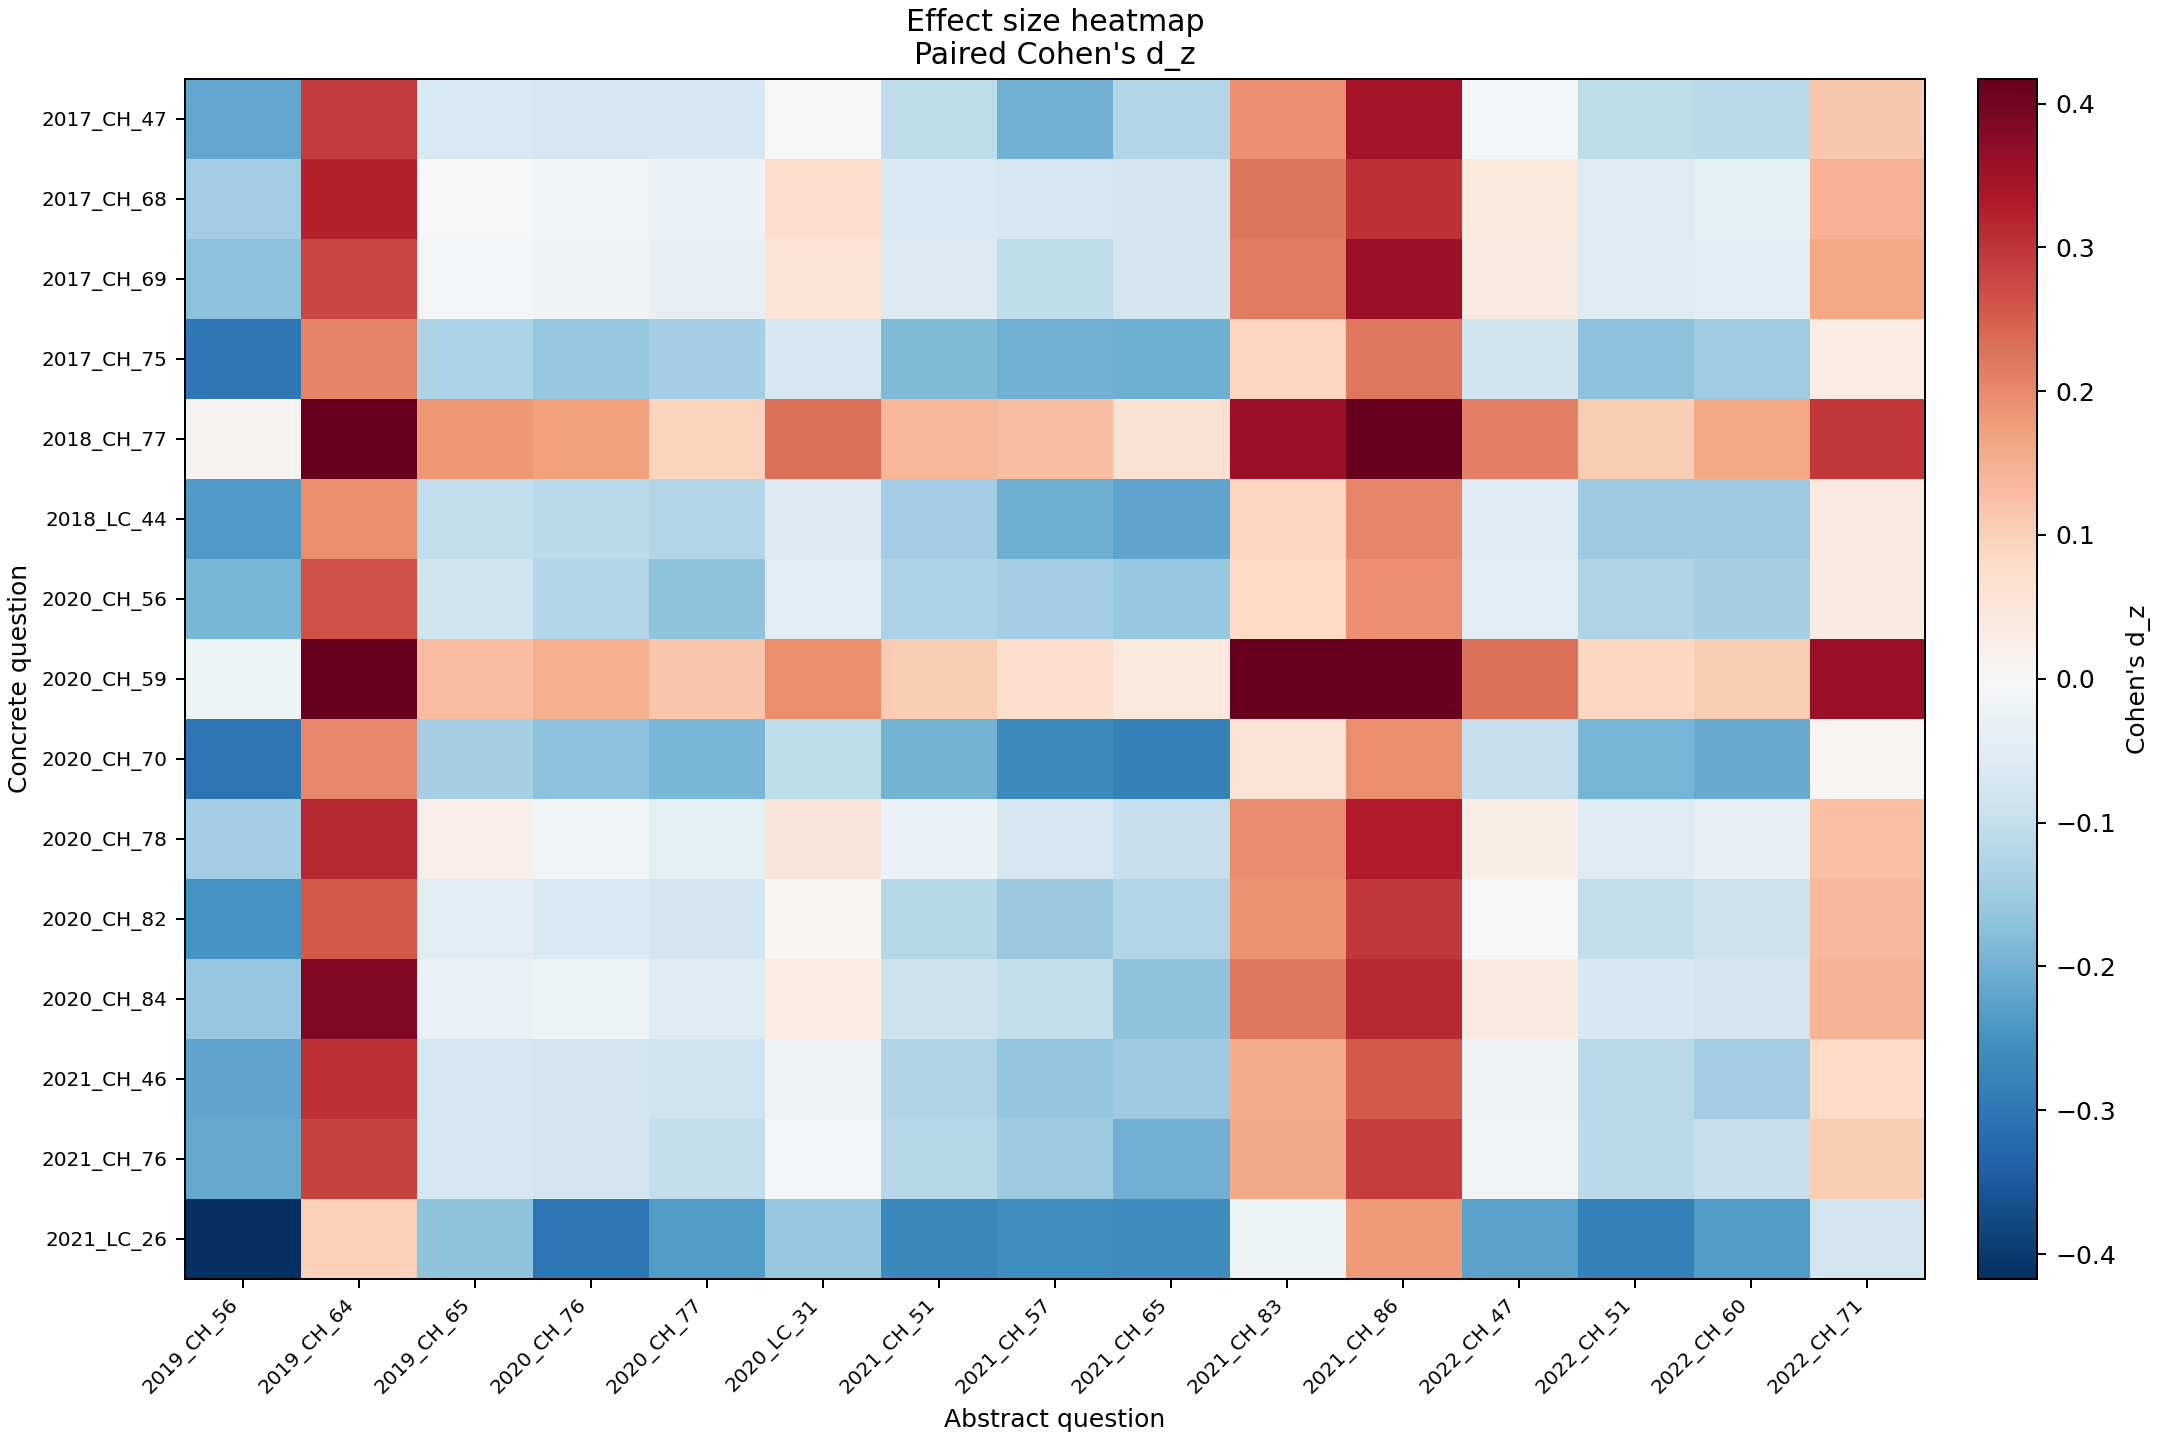
\includegraphics[width=0.48\linewidth]{../../figures/step8/pairwise_effect_size_heatmap.png}
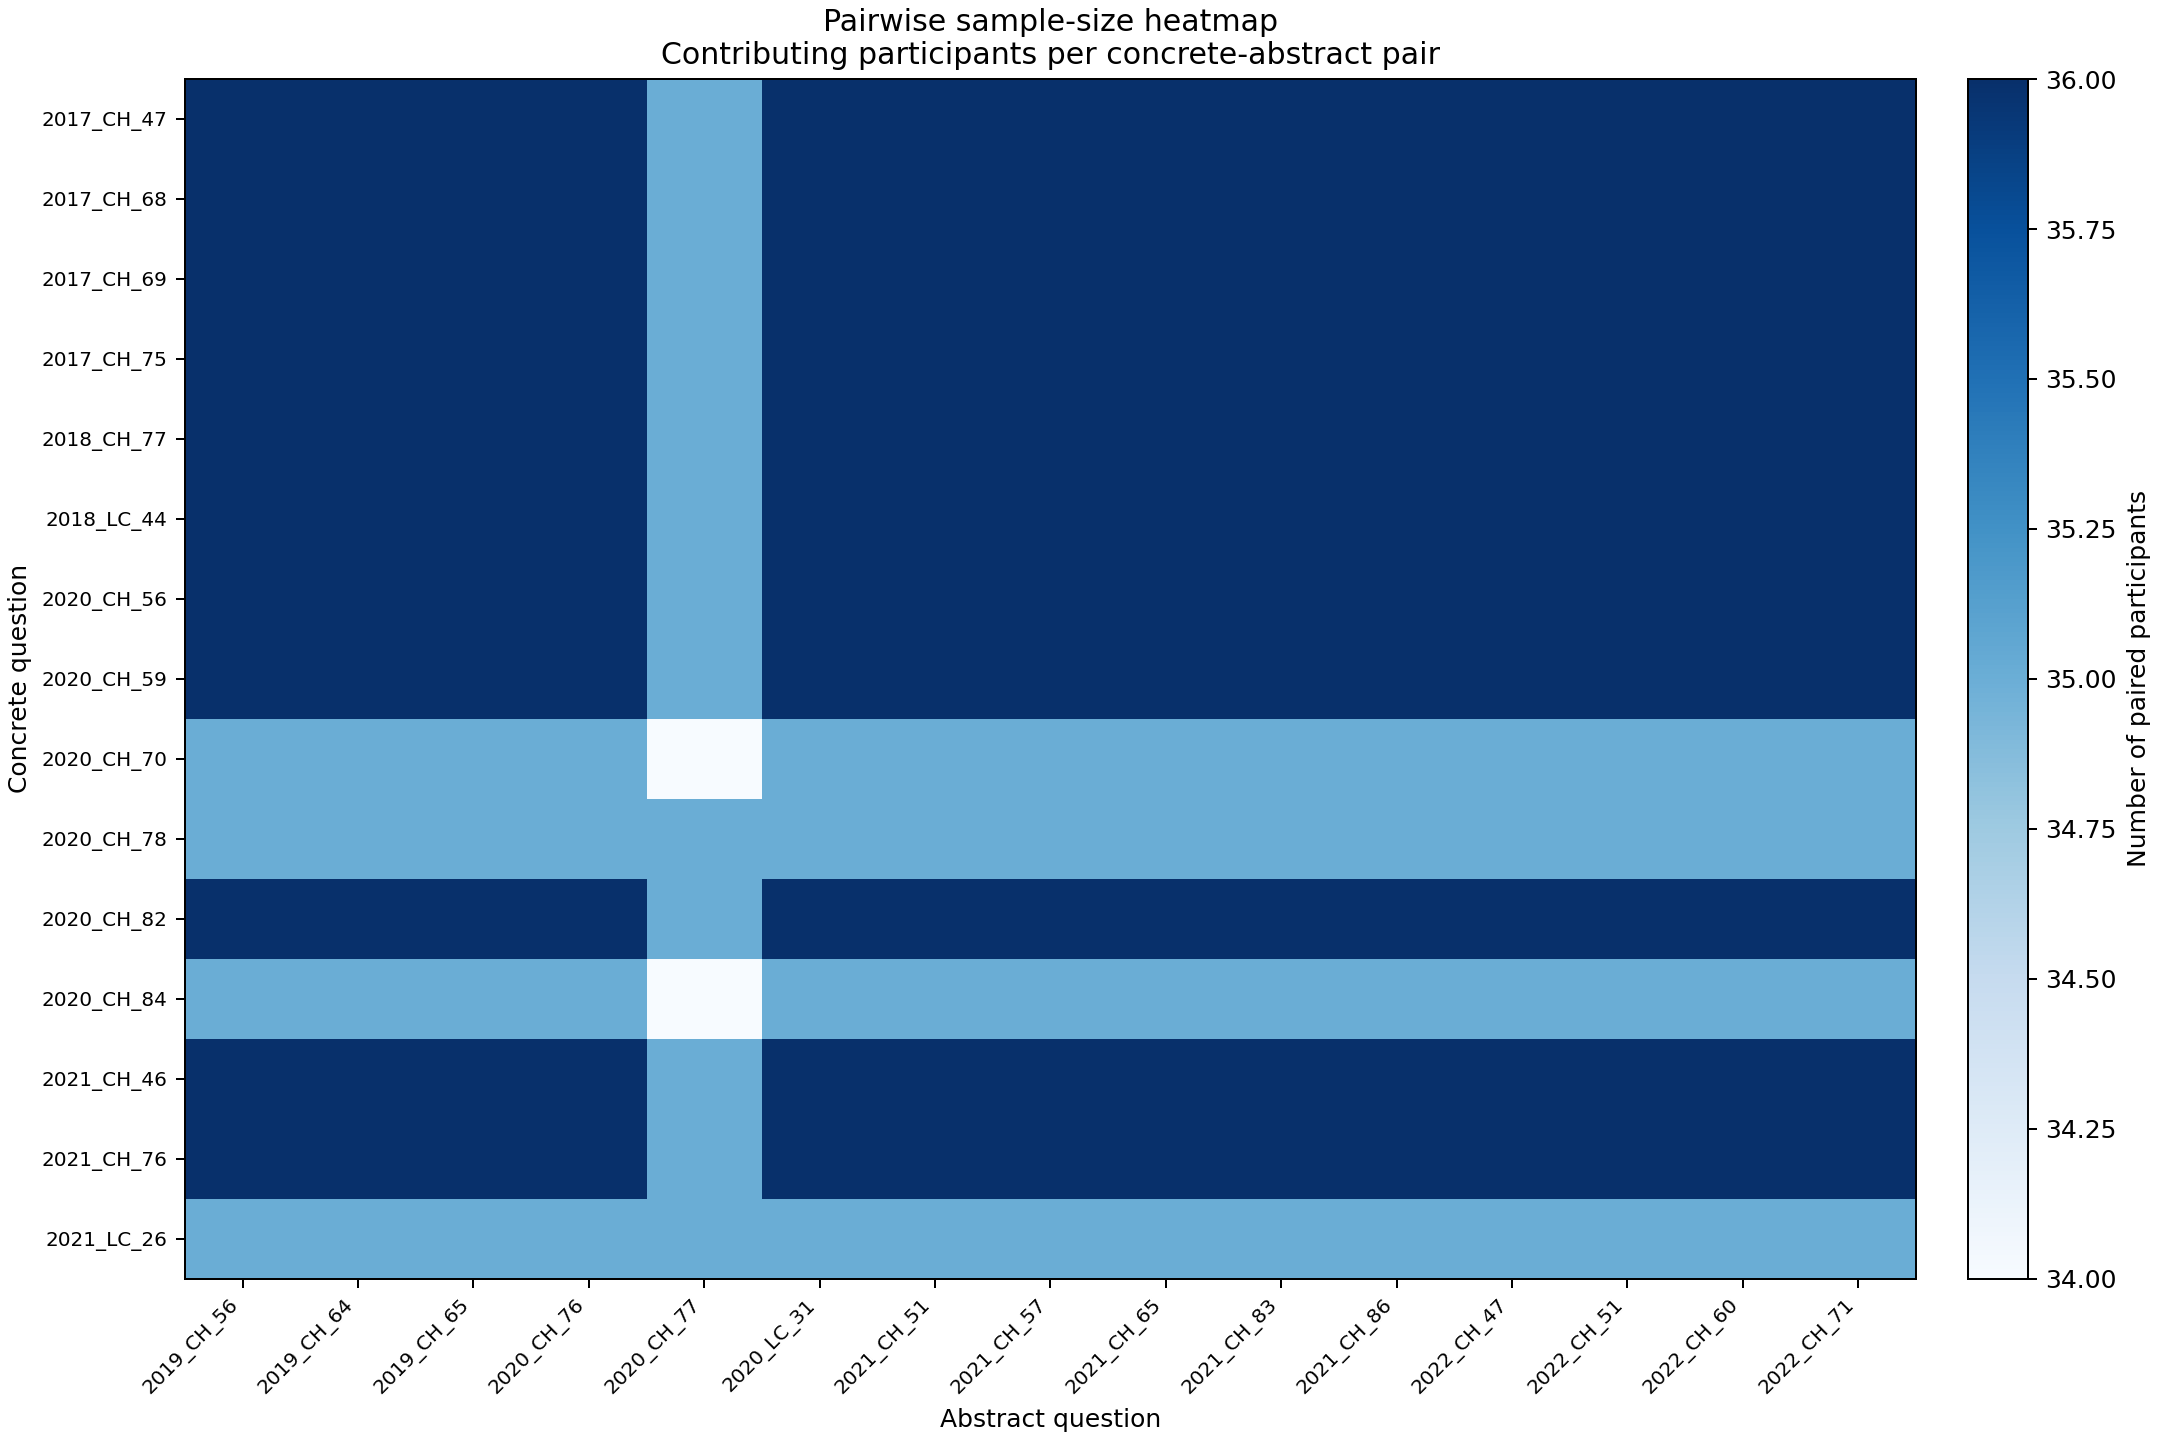
\includegraphics[width=0.48\linewidth]{../../figures/step8_visualization/pairwise_sample_size_heatmap.png}
\caption{Paired effect sizes and the contributing sample size for each concrete-abstract pair.}
\end{figure}
\subsection*{Descriptive Ranking Views}
\begin{figure}[H]
\centering
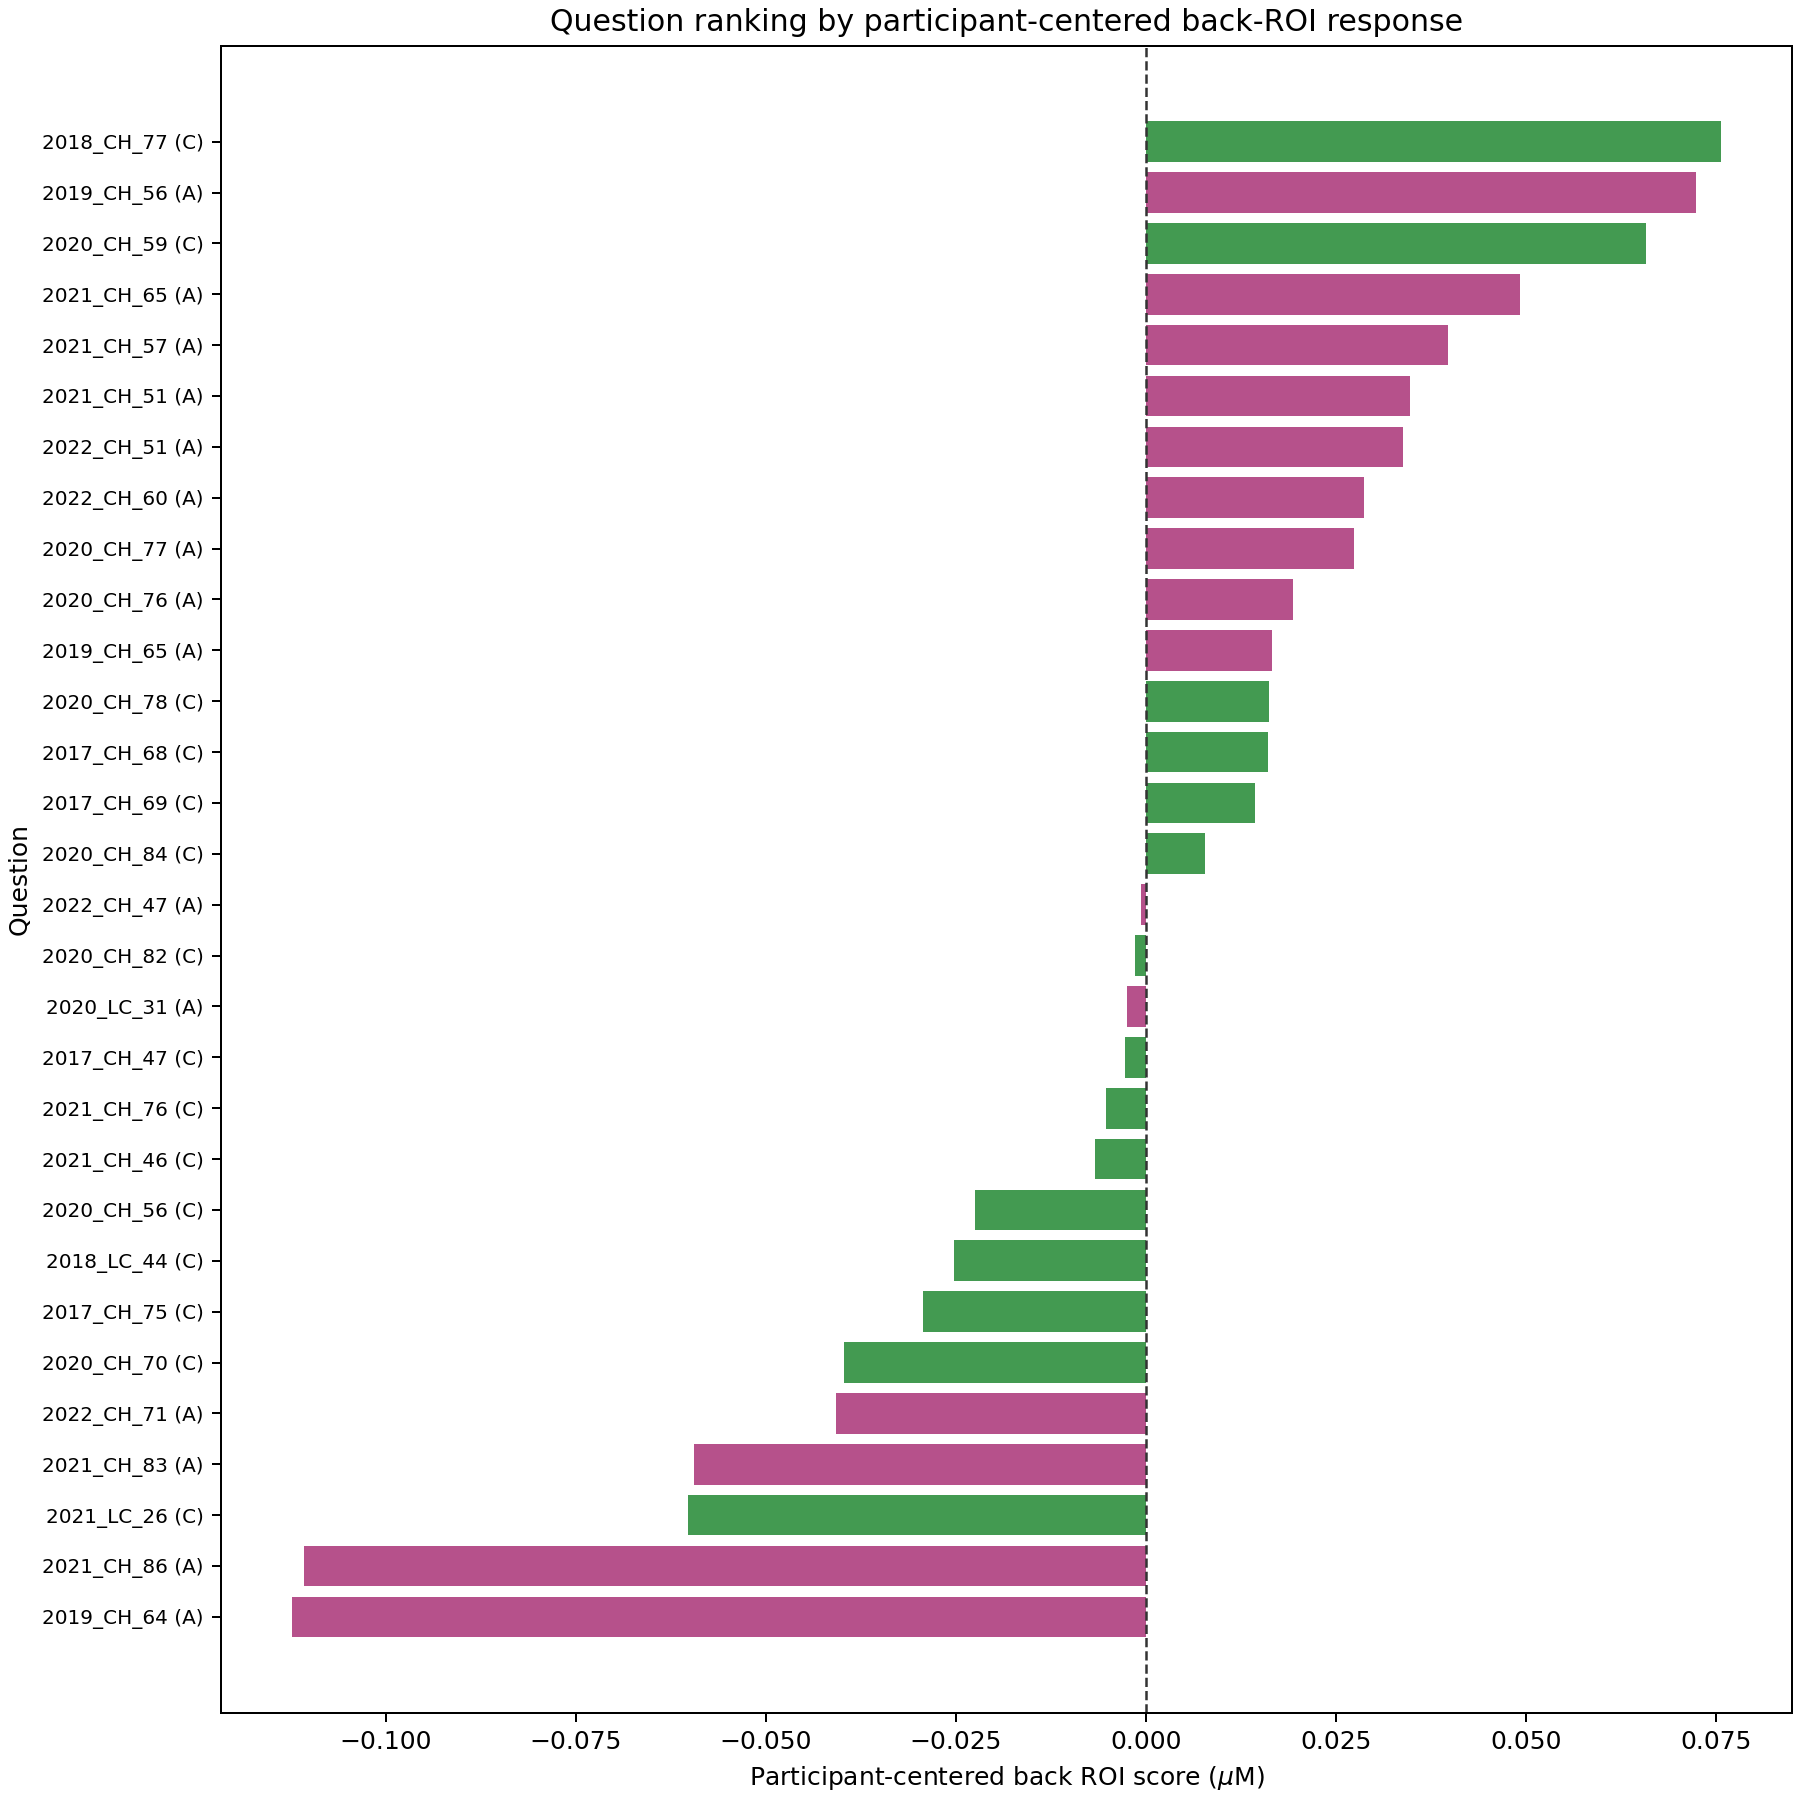
\includegraphics[width=0.90\linewidth]{../../figures/step8/question_centered_ranking_plot.png}
\caption{Participant-centered ranking of questions by back-ROI response.}
\end{figure}
\begin{figure}[H]
\centering

\includegraphics[width=0.92\linewidth]{../../figures/step8_visualization/top_pair_forest_plot.png}
\caption{Top descriptive item pairs ranked by the strongest pairwise evidence, shown with mean differences and 95\% confidence intervals.}
\end{figure}
\subsection*{Matching And Channel Follow-up}
\begin{figure}[H]
\centering
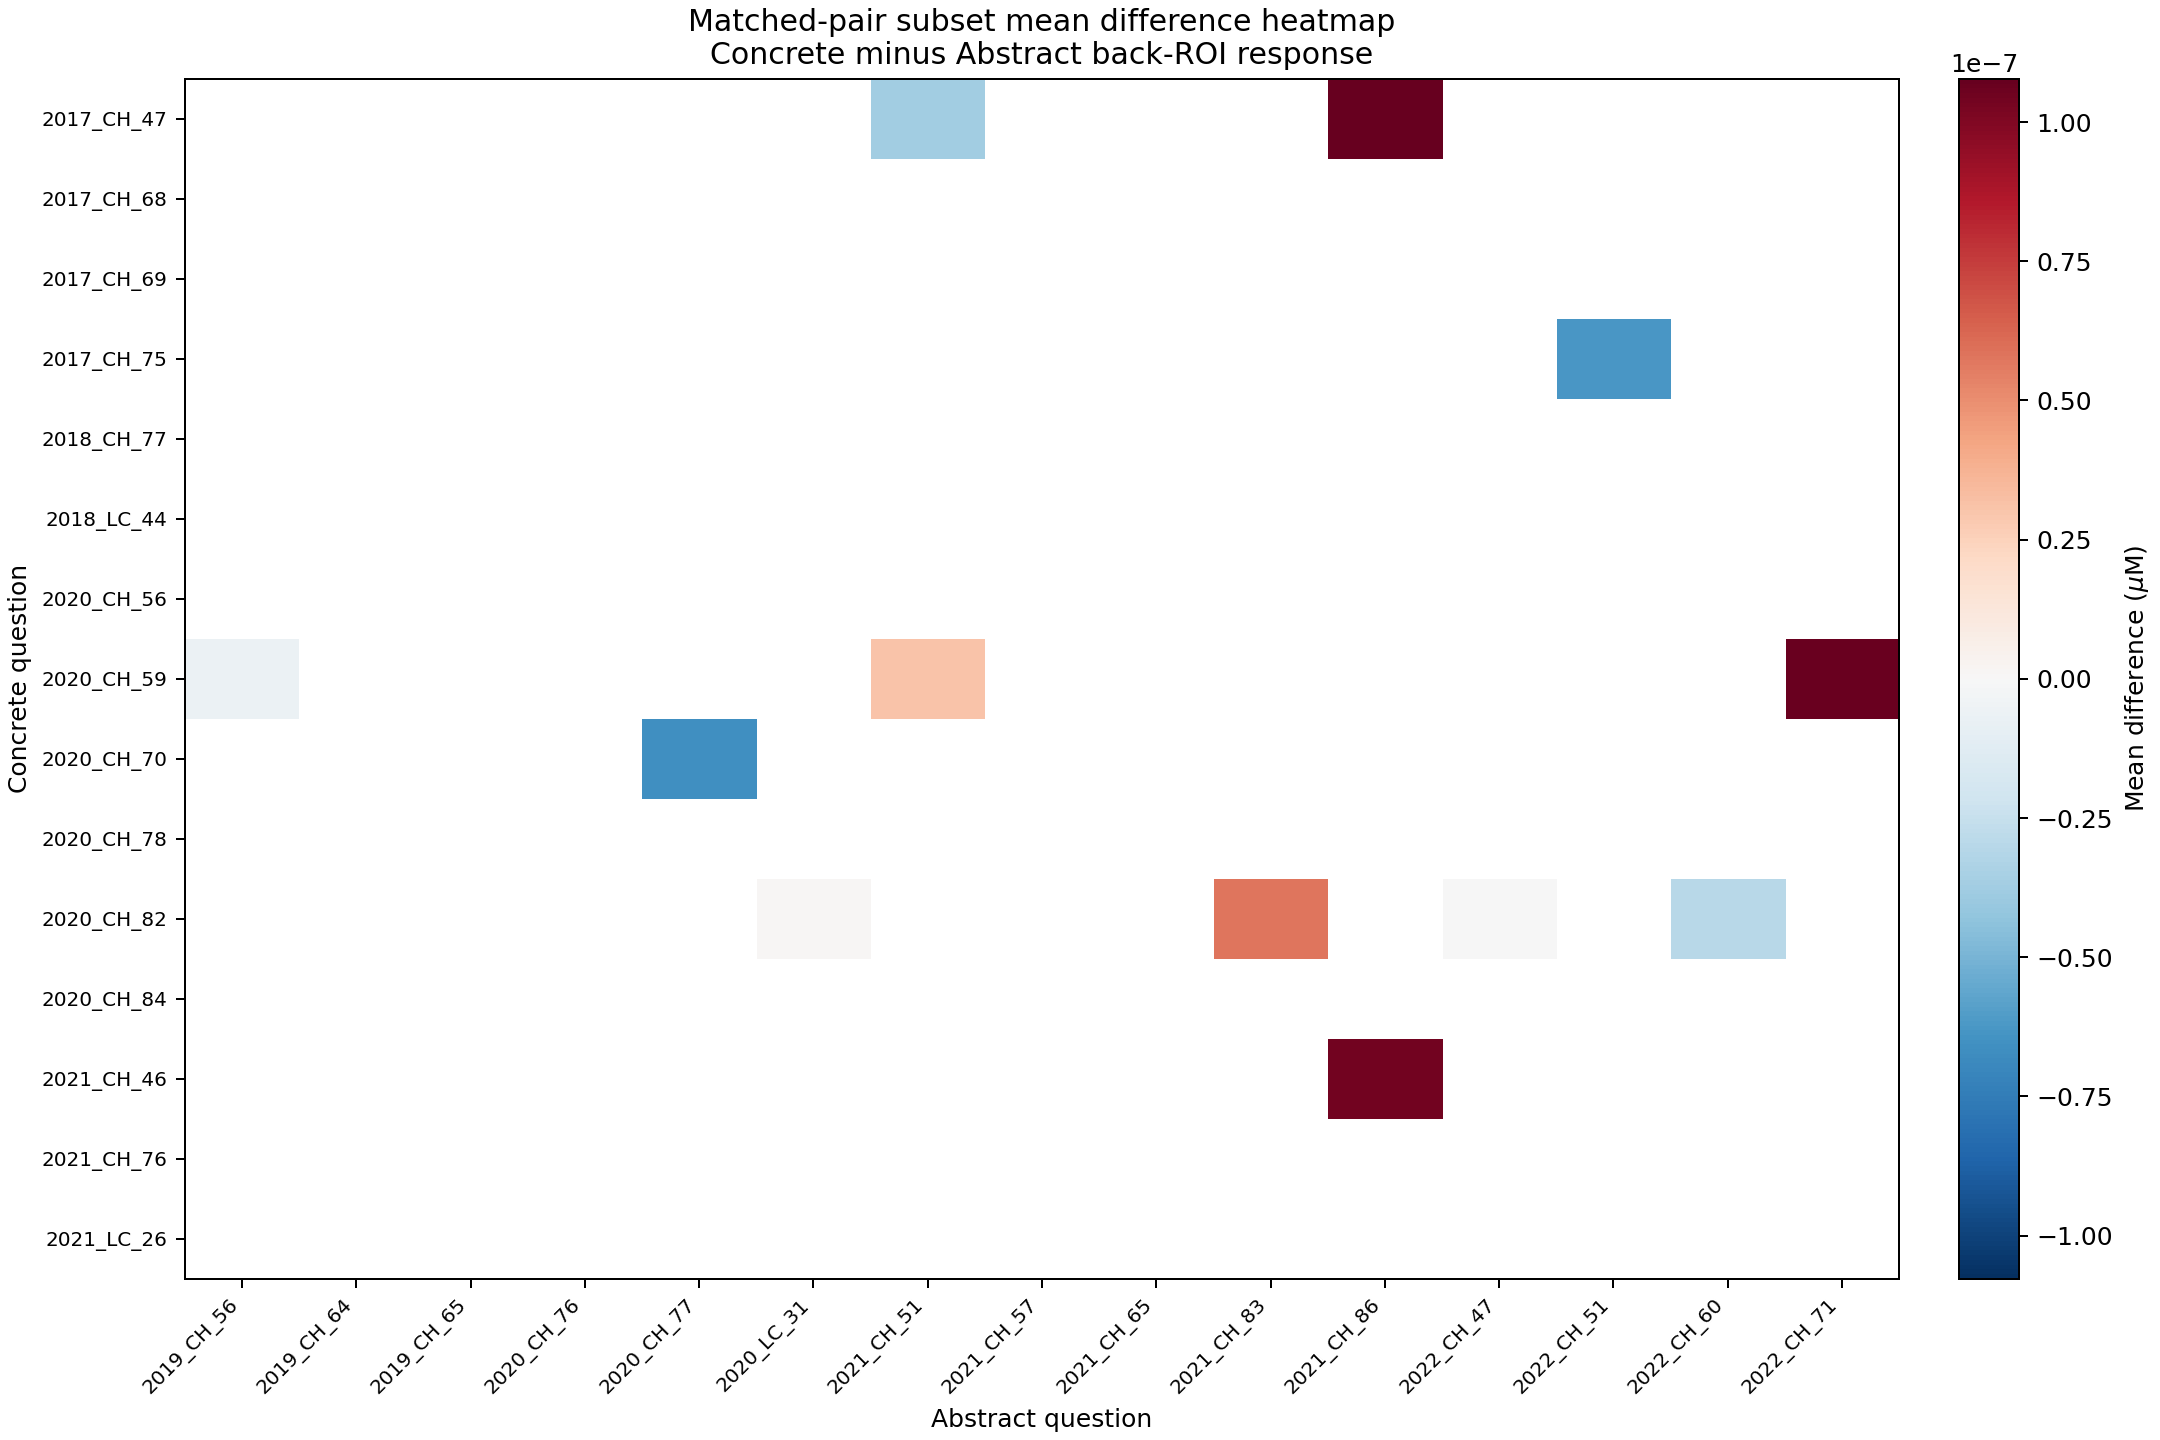
\includegraphics[width=0.48\linewidth]{../../figures/step8/matched_pair_heatmap.png}
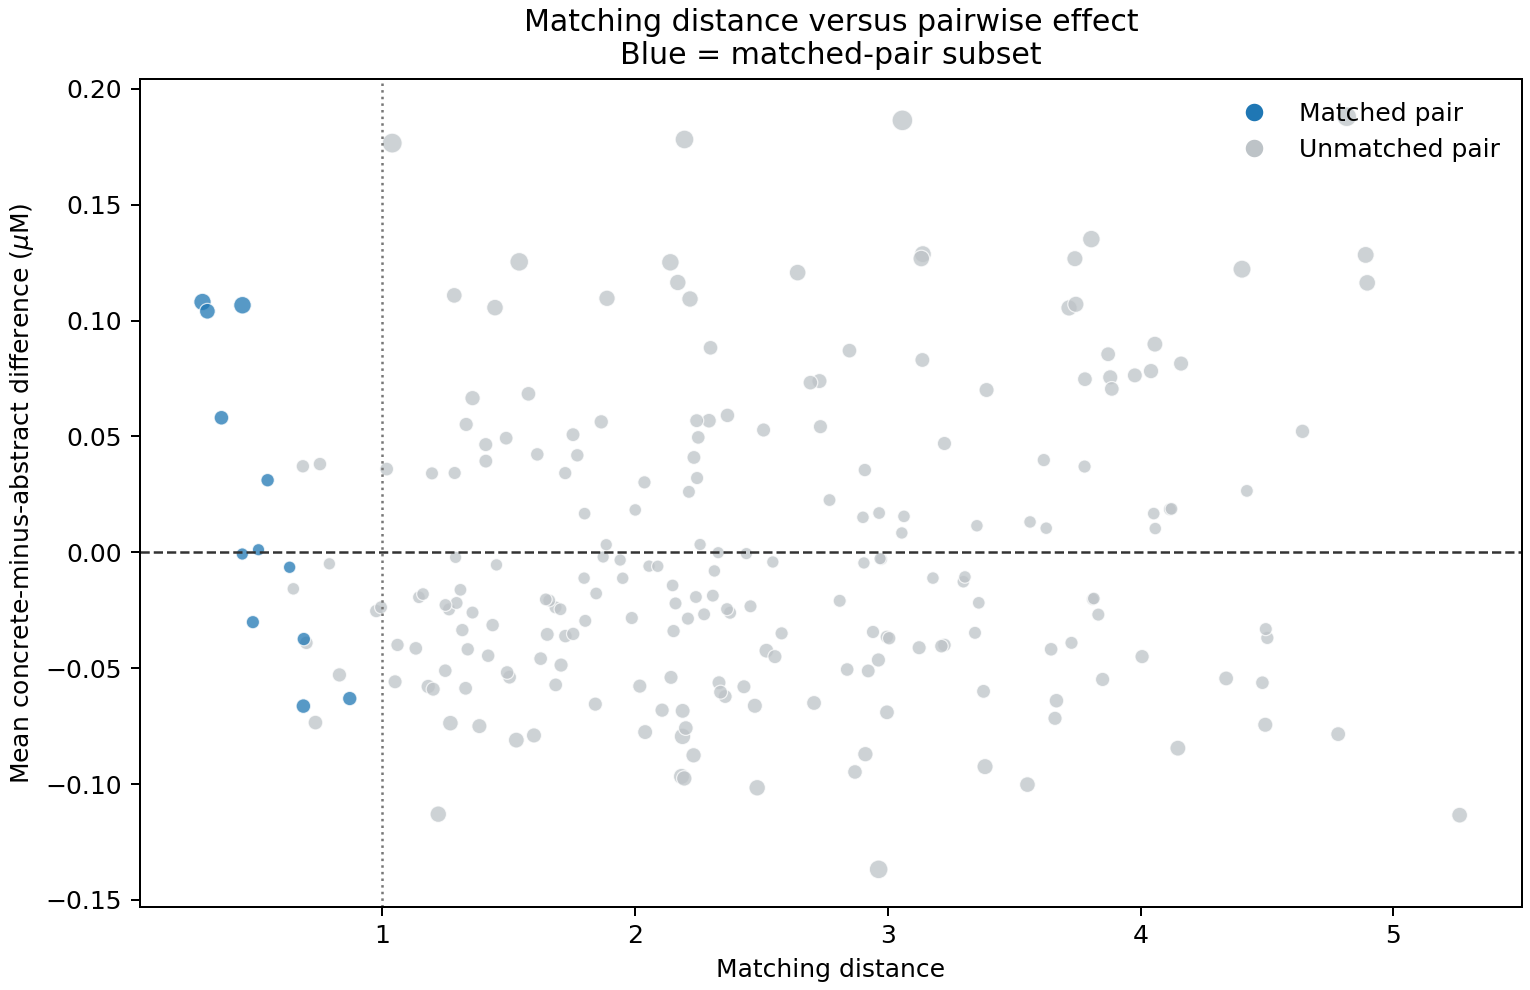
\includegraphics[width=0.48\linewidth]{../../figures/step8_visualization/matching_distance_scatter.png}
\caption{Matched-pair subset heatmap and the relation between matching distance and pairwise mean effect.}
\end{figure}
\begin{figure}[H]
\centering
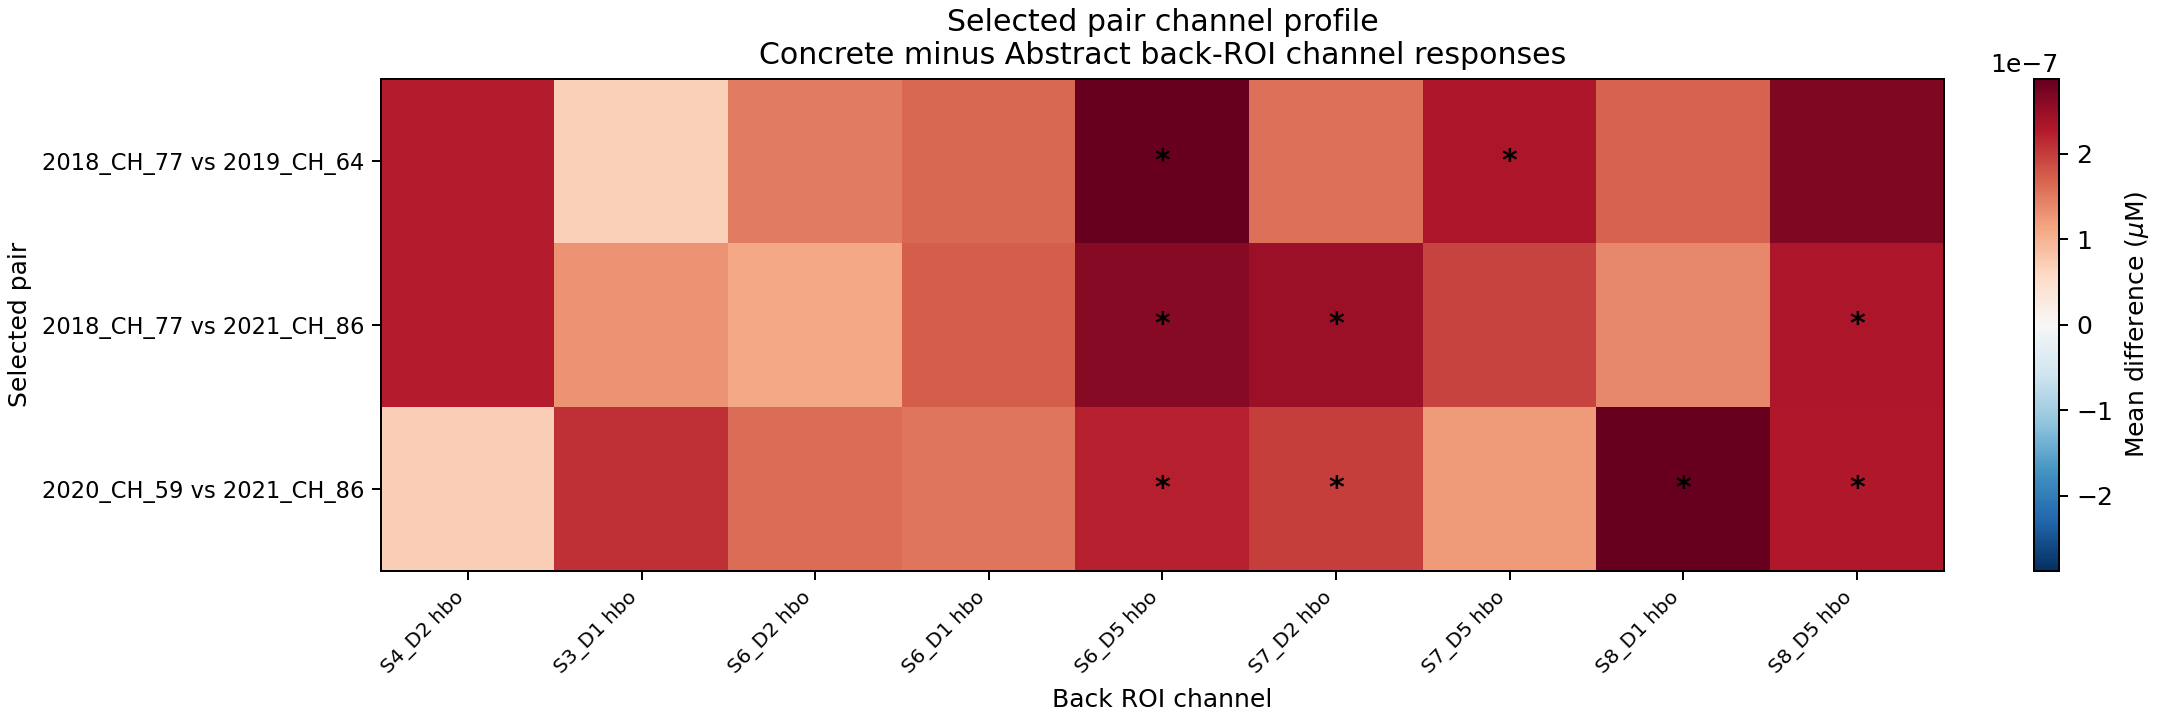
\includegraphics[width=0.95\linewidth]{../../figures/step8/selected_pair_channel_profile.png}
\caption{Optional back-channel follow-up for the selected descriptive pairs.}
\end{figure}
\end{document}
